\subsection[Umsetzung eines filterbasierten Systemes]{Umsetzung eines filterbasierten Systemes am Beispiel von Mercury}
\label{chap:related:mercury}
Im System von Mercury \cite{Bharambe2004Mercury} gibt es ein Set von Attributen, die ihrerseits einen definierten Wertebereich haben. Mercury limitiert die Datentypen auf Zahlen und Strings. In \Fref{fig:mercury} ist sind dies \enquote{x'' und ``y} mit je einem Intervall ganzer Zahlen als Wertebereich. Jedes Attribut wird durch einen eigenen Verbund aus Knoten, dem sogenannten \emph{Hub}, bearbeitet. Der Wertebereich ist dabei nicht zwingend symmetrisch auf die Knoten verteilt, wie in der Grafik durch die verschiedenen Größen der Kreissegmente dargestellt ist. 

\begin{figure}[htbp]
\centering
\resizebox{\textwidth}{!}{%
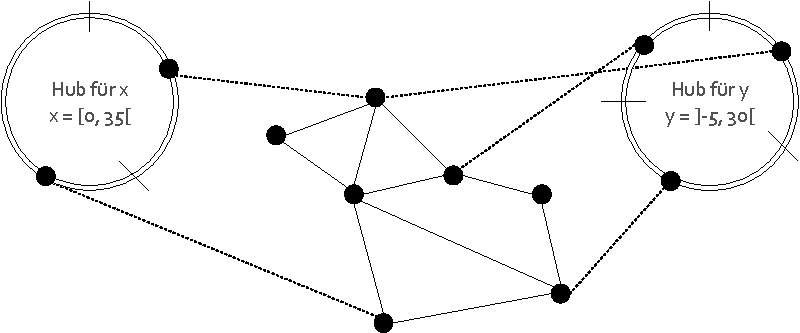
\includegraphics{grafics/mercury.pdf}}
\caption{Aufbau von Mercury}
\label{fig:mercury}
\end{figure}

\paragraph{Subscribe}
Eine Subscription $S$ ist ein Tupel aus Filterbedingungen über die Attribute, zum Beispiel $S := (5 < x <= 20; y = 15)$, sowie Kontaktinformationen des Knotens. Für jede Subscribtion wird das Attribut mit der größten Selektivität ausgewählt; im Beispiel ist dies Attribut $y$. $S$ wird nun an einen beliebigen Knoten aus dem zuständigen Hubs gesendet. Im Hub wird $S$ nun zu dem Knoten weitergereicht, der den Wertebereich der Filterung abdeckt und dort in einer Liste gespeichert. Es ist ebenso möglich, dass eine Anmeldung -- je nach abgedecktem Wertebereich -- bei mehreren Knoten abgespeichert wird.

\paragraph{Unsubscribe}
Zur Abmeldung muss ein entsprechendes \enquote{Negativ}-Tupel zur Anmeldung an den selben Hub wie das Anmeldetupel gesendet werden. Am richtigen Knoten angekommen, wird der Listeneintrag entfernt.

\paragraph{Publish}
Eine Publikation $P$ ist ebenfalls ein Tupel mit bestimmten Werten der Attribute, wie zum Beispiel $P := (x = 10; y = 0)$. Im Unterschied zur Anmeldung wird eine Publikation an \emph{alle} Hubs gesendet und dort zum jeweils zuständigen Knoten weitergereicht. Dieser gleicht $P$ mit den gespeicherten Anmeldetupel ab und senden $P$ an den zugehörigen Knoten.

Mirinae ist ebenfalls ein filterbasiertes Publish/Subscribe-System, stellt den Wertebereich eines Attributes jedoch als Hyperwürfel dar. Eine automatische Anpassung dieser Aufteilung ermöglicht eine schnelle Anpassung der Routingtabelle und damit einen kurzen Weg für die Nachrichten \cite{Choi2005Mirinae}.
